\documentclass[a4paper,12pt]{report}
\usepackage[T2A]{fontenc}
\usepackage[utf8]{inputenc}
\usepackage[english,russian]{babel}
\usepackage{graphicx}
\usepackage{wrapfig}
\usepackage{float}
\restylefloat{table}
\usepackage{mathtext} 				% русские буквы в фомулах
\usepackage{amsmath,amsfonts,amssymb,amsthm,mathtools} % AMS
\usepackage{icomma} % "Умная" запятая: $0,2$ --- число, $0, 2$ --- перечисление
\usepackage{capt-of}
\usepackage{appendix}
\usepackage{multirow}
\usepackage{hyperref}
\usepackage[left=2cm,right=2cm,
    top=2cm,bottom=2cm,bindingoffset=0cm]{geometry}
\usepackage{multicol} % Несколько колонок
\usepackage{gensymb}
\title{Отчёт по лабораторной работе №4.2.1 

Кольца Ньютона.}
\author{Плюскова Н.А. Б04-004 }
\date{\today}

\begin{document}

\maketitle

\section*{\huge{Описание работы}}
\noindent\textbf{Цель работы:} познакомиться с явлением интерференции в тонких плёнках (полосы равной толщины) на примере колец Ньютона и с методикой интерференционных измерений кривизны стеклянной поверхности.

\noindent\textbf{В работе используются:} измерительный микроскоп с опак-иллюминатором, плоско-выпуклая линза; пластинка из чёрного стекла, ртутная лампа типа ДРШ, щель, линзы, призма прямого зрения, объектная шкала.

\subsection*{Аннотация}
В работе предлагается, измерив диаметры колец Ньютона, определить радиус кривизны линзы; исследовать картину биений и рассчитать разность длин волн между желтой и зеленой спектральными линиями ртути.

\subsection*{Теоретические сведения}

	\begin{wrapfigure}{l}{0.35\linewidth} 
		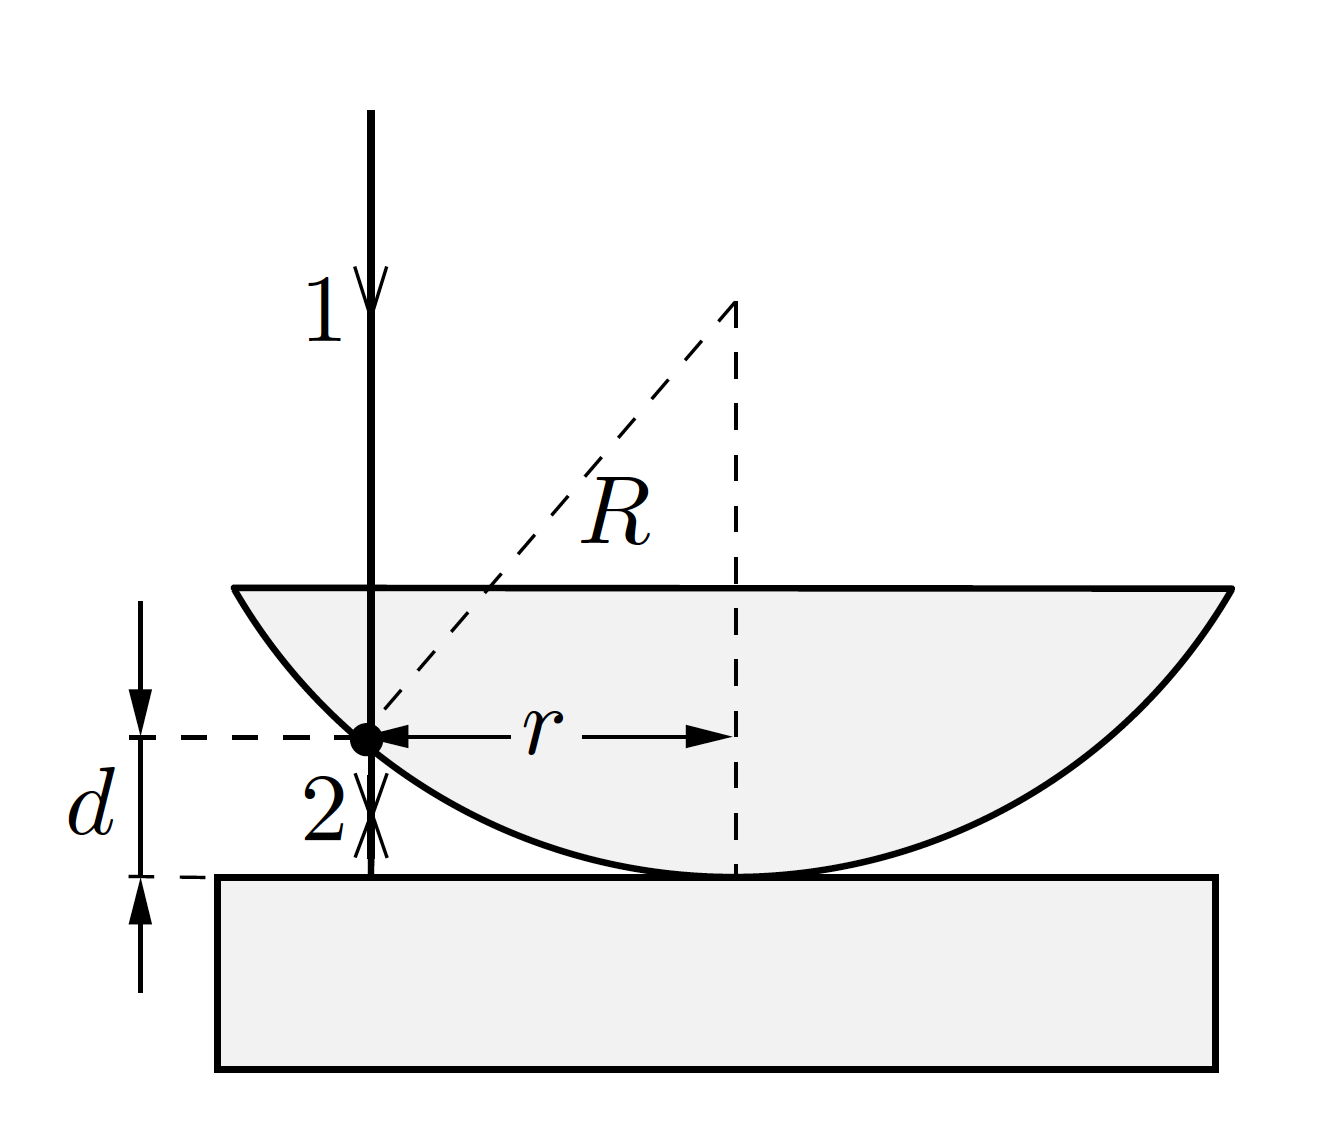
\includegraphics[width=\linewidth]{ring}
		\caption{Экспериментальная установка}
		\label{ring}
	\end{wrapfigure}

	Этот классический опыт используется для определения радиуса кривизны сферических поверхностей линз. В этом опыте наблюдается интерференция волн, отражённых от границ тонкой воздушной прослойки, образованной сферической поверхностью линзы и плоской стеклянной пластиной. При нормальном падении света (рис. \ref{ring}) интерференционные полосы локализованы на сферической поверхности и являются полосами равной толщины.
	
	Геометрическая разность хода между интерферирующими лучами равна удвоенной толщине воздушного зазора $ 2d $ в данном месте. Для точки на сферической поверхности, находящейся на расстоянии $ r $ от оси системы, имеем $ r^2 = R^2 - (R - d)^2 = 2Rd - d^2 $, где $ R $ --- радиус кривизны сферической поверхности (рис. \ref{ring}).
	
	При $ R \gg d $ получим$  d = r^2/2R $. С учётом изменения фазы на $ \pi $ при отражении волны от оптически более плотной среды (на границе воздух-стекло) получим \textbf{оптическую разность хода интерферирующих лучей}:
	
	\begin{equation}\label{r_m}
	\Delta = \dfrac{\lambda}{2} + 2d = \dfrac{r^2}{2R} + \dfrac{\lambda}{2}
	\end{equation}
	
	Из условия интерференционного минимума $ \Delta = \dfrac{(2m +1)\lambda}{2}, \; m =0, 1, 2.. $ получим радиусы темных колец $ r_m $, а из аналогичного условия максимума $ \Delta = m \lambda $ радиусы светлых $ r_m' $ :
	
	\begin{equation}\label{r_m'}
	r_m = \sqrt{m \lambda R}, \qquad 	r_m' = \sqrt{\dfrac{(2m-1)m \lambda R}{2}}
	\end{equation}
\subsection*{Экспериментальная установка} 

Схема экспериментальной установки приведена на рис. \ref{lab}. Опыт выполняется с помощью измерительного микроскопа.
На столик микроскопа помещается держатель с полированной пластинкой из
чёрного стекла. На пластинке лежит исследуемая линза.
\newpage

	\begin{wrapfigure}{r}{0.5\linewidth} 
	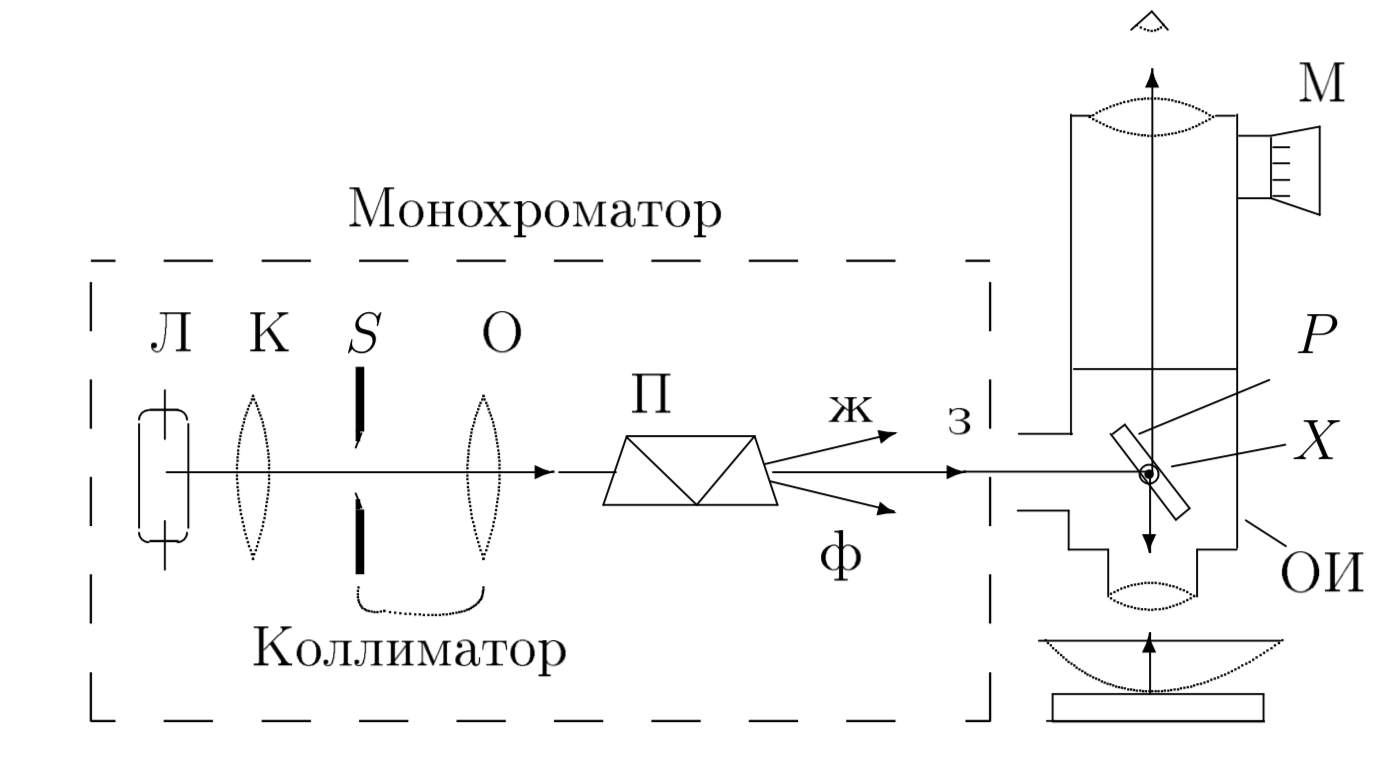
\includegraphics[width=\linewidth]{lab}
	\caption{Экспериментальная установка}
	\label{lab}
\end{wrapfigure}

	Источником света служит ртутная лампа, находящаяся в защитном кожухе. Для получения монохроматического света применяется призменный монохроматор, состоящий из конденсора $ К $, коллиматора (щель $ S $ и объектив $ О $) и призмы прямого зрения $ П $. Эти устройства с помощью рейтеров располагаются на оптической скамье. Свет от монохроматора попадает на расположенный между объективом и окуляром микроскопа опак-иллюминатор (ОИ)  специальное устройство, служащее для освещения объекта при работе в отражённом свете. Внутри опак-иллюминатора находится полупрозрачная стеклянная пластинка P, наклоненная под углом $ 45^\circ $ к оптической оси микроскопа. Свет частично отражается от этой пластинки, проходит через объектив микроскопа и попадает на исследуемый объект. Пластинка может поворачиваться вокруг горизонтальной оси $ X $, опак-иллюминатор вокруг вертикальной оси.

	Столик микроскопа может перемещаться в двух взаимно перпендикулярных направлениях помощью винтов препаратоводителя. Отсчетный крест окулярной шкалы перемещается перпендикулярно оптической оси с помощью микрометрического винта $ М $.
	
	Оптическая схема монохроматора позволяет получить в плоскости входного окна опак-иллюминатора достаточно хорошо разделённые линии спектра ртутной лампы. Изображение щели $ S $ фокусируется на поверхность линзы объективом микроскопа, т.е. точка источника и точка наблюдения спектра совпадают.Интерференционная картина не зависит от показателя преломления линзы и определяется величиной зазора между линзой и пластинкой (кольца равной толщины).

	Сначала микроскоп настраивается на кольца Ньютона в белом свете (свете ртутной лампы), затем при помощи монохроматора выделить из спектра яркую зелёную линию и провести измерения диаметров колец в монохроматическом свете. 
	

\newpage
\section*{\huge{Выполнение работы}}

\vspace{\baselineskip}
\noindent\textbf{I. Калибровка окулярной шкалы}

Определим цену деления окулярной шкалы: 4.43 деления окулярной шкалы 0.4 мм. Следовательно, цена деления окулярной шкалы: $\Delta x = (91 \pm 2)*10^(-6)$ м.

\noindent\textbf{II. Измерение диаметров колец}

После настройки микроскопа проведем измерения диаметров колец Ньютона. Измерения будем проводить в безразмерных единицах окулярной шкалы, переведённых затем в реальную величину с помощью калиброванной объектной шкалы. 
	
	
	Оценим систематическую погрешность измерения величин на окуляре как $ \sigma = 0,01 $ 
	
	C помощью светофильтра получим желтый цвет ($ \lambda = 576 $ нм), в котором и будет производить замеры диаметров колец Ньютона.
	
	Перемещая перекрестие, последовательно устанавливаем его на середины темных колец и записываем соответствующие показания $x_1$ окулярной шкалы и микрометра. После прохождения через центральное пятно продолжаем измерения, записывая возрастающие номера колец и координаты $x_2$ их диаметров. Для устранения ошибок, возникающих из-за люфта в винте, перекрестие всегда следует подводить к кольцу с одной стороны.


\begin{table}[H]
\centering
\begin{tabular}{|c|ccc|ccc|}
\hline
\multirow{2}{*}{m} & \multicolumn{3}{c|}{\textbf{Темные кольца}}                                                         & \multicolumn{3}{c|}{\textbf{Светлые кольца}}                                                        \\ \cline{2-7} 
                   & \multicolumn{1}{l|}{$x_{1}$, усл.ед} & \multicolumn{1}{l|}{$x_{2}$, усл.ед} & \multicolumn{1}{l|}{$r_{m}$, усл.ед} & \multicolumn{1}{l|}{$x_{1}$, усл.ед} & \multicolumn{1}{l|}{$x_{2}$, усл.ед} & \multicolumn{1}{l|}{$r_{m}$, усл.ед} \\ \hline
1                  & \multicolumn{1}{c|}{2,5}        & \multicolumn{1}{c|}{4,12}       & 1,62                            & \multicolumn{1}{c|}{2,42}       & \multicolumn{1}{c|}{3,71}       & 1,29                            \\ \hline
2                  & \multicolumn{1}{c|}{1,77}       & \multicolumn{1}{c|}{4,51}       & 2,74                            & \multicolumn{1}{c|}{1,98}       & \multicolumn{1}{c|}{4,33}       & 2,35                            \\ \hline
3                  & \multicolumn{1}{c|}{1,51}       & \multicolumn{1}{c|}{4,79}       & 3,28                            & \multicolumn{1}{c|}{1,63}       & \multicolumn{1}{c|}{4,63}       & 3                               \\ \hline
4                  & \multicolumn{1}{c|}{1,23}       & \multicolumn{1}{c|}{5,7}        & 4,47                            & \multicolumn{1}{c|}{1,39}       & \multicolumn{1}{c|}{4,98}       & 3,59                            \\ \hline
5                  & \multicolumn{1}{c|}{0,87}       & \multicolumn{1}{c|}{5,31}       & 4,44                            & \multicolumn{1}{c|}{1,91}       & \multicolumn{1}{c|}{5,18}       & 3,27                            \\ \hline
6                  & \multicolumn{1}{c|}{0,64}       & \multicolumn{1}{c|}{5,48}       & 4,84                            & \multicolumn{1}{c|}{0,73}       & \multicolumn{1}{c|}{5,39}       & 4,66                            \\ \hline
7                  & \multicolumn{1}{c|}{0,51}       & \multicolumn{1}{c|}{5,67}       & 5,16                            & \multicolumn{1}{c|}{0,57}       & \multicolumn{1}{c|}{5,56}       & 4,99                            \\ \hline
8                  & \multicolumn{1}{c|}{0,35}       & \multicolumn{1}{c|}{5,83}       & 5,48                            & \multicolumn{1}{c|}{0,43}       & \multicolumn{1}{c|}{5,76}       & 5,33                            \\ \hline
9                  & \multicolumn{1}{c|}{0,21}       & \multicolumn{1}{c|}{6,01}       & 5,8                             & \multicolumn{1}{c|}{0,29}       & \multicolumn{1}{c|}{5,94}       & 5,65                            \\ \hline
10                 & \multicolumn{1}{c|}{0,13}       & \multicolumn{1}{c|}{6,16}       & 6,03                            & \multicolumn{1}{c|}{0,14}       & \multicolumn{1}{c|}{6,1}        & 5,96                            \\ \hline
\end{tabular}
\caption{Измерение диаметров колец Ньютона}
\end{table}

\begin{center}
    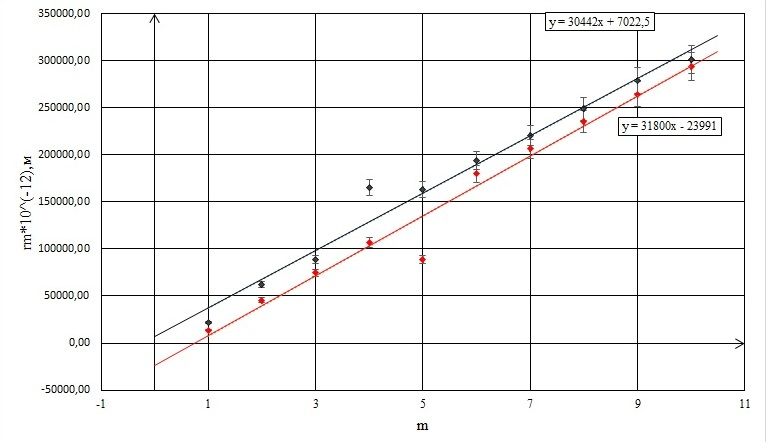
\includegraphics[width = \linewidth]{graph.jpg}
    \captionof{figure}{График зависимости радиусов колец от их номера. Значения коэффициентов наклона: $k_{max} = 3.18\cdot 10^{-9} \text{м};$  
      $ k_{min} = 3.04\cdot 10^{-9} \text{м}.$}
\end{center}

Найдем коэффициент наклона касательной:
\begin{equation*}
    k = \sqrt{\frac{<xy>-<x>\cdot<y>}{<x^2>-<x>}}
\end{equation*}
\begin{equation*}
    \sigma_k = \sqrt{\frac{1}{n-1}(\frac{<y^2>}{<x^2>}-k^2)}
\end{equation*}

\begin{equation*}
    k_{max} = (7,95\pm 0,09)\cdot10^{-9} \text{м}
\end{equation*}
\begin{equation*}
    k_{min} = (7,61\pm 0,1)\cdot10^{-9} \text{м}
\end{equation*}
Из формул $r_{m} = \sqrt{m\lambda R}$ и $r'_{m} = \sqrt{(2m - 1)m\lambda R/2}$ найдем значения радиуса кривизны линзы:
\begin{equation*}
    R_{max} = \frac{k_{max}}{\lambda} = \frac{7.95 \cdot 10^{-9}}{579 \cdot 10^{-9}} = 13.73 \pm 0.16 \text{ мм} 
\end{equation*}

\begin{equation*}
    R_{min} = \frac{k_{min}}{\lambda} = \frac{7.61 \cdot 10^{-9}}{579 \cdot 10^{-9}} = 13.14 \pm 0.15 \text{ мм} 
\end{equation*}
	
\vspace{\baselineskip}
\noindent\textbf{III. "Наблюдение биений"}

Убрав светофильтр, в опак-иллюминатор поступает свет от ртутной лампы, в спектре которой преобладают желтый и зеленый цвета. Из-за того, что волны желтого и зеленого лучей имеют разную длину волны, мы видим картину биений - череду четких и нечетких систем колец.

Посчитаем количество темных полос между соседними четкими системами: $\delta m = 16$. Зная длину волны желтого света $\lambda_{y}$, мы можем определить длину волны зеленого свет$\lambda_{g}$а и разность длин волн желтого и зеленого света ртутной лампы.

\begin{equation*}
    \lambda_{y}m=\lambda_{g}(m+1) \rightarrow m+1 =\frac{\lambda_{y}}{\Delta\lambda}
\end{equation*}

\begin{equation*}
    \Delta\lambda=\frac{\lambda_{y}}{m+1} = \frac{574 \text{ нм}}{17} \approx 34 \text{ нм}
\end{equation*}

\section*{Вывод}

В данной работе было изучено явление интерференции в тонких пленках - кольца Ньютона, получено значение радиуса кривизны линзы:

\begin{equation*}
    < R > = 13.43 \pm 0.16 \text{ мм}
\end{equation*}
Определили из экспериментального периода биений разницу длин волн зеленого и желтого света ртутной лампы ($\Delta\lambda \approx 34 $ нм), которое практически совпадает с табличным значением - 33 нм.

\end{document}
